%% Mixed-Precision Project Pipeline Diagram
%% Compile with: pdflatex project_pipeline.tex
%%
\documentclass[border=10pt]{standalone}
\usepackage{tikz}
\usetikzlibrary{positioning, fit, arrows.meta, calc, shapes.geometric, backgrounds, decorations.pathreplacing}
\usepackage{xcolor}
\usepackage{pifont}

% Color palette
\definecolor{swRed}{HTML}{E94560}
\definecolor{swRedLt}{HTML}{FDE8EC}
\definecolor{hwBlue}{HTML}{0F3460}
\definecolor{hwBlueLt}{HTML}{E0E8F0}
\definecolor{verGreen}{HTML}{16C79A}
\definecolor{verGreenLt}{HTML}{D6F5EC}
\definecolor{arrowGray}{HTML}{6B7280}

\begin{document}
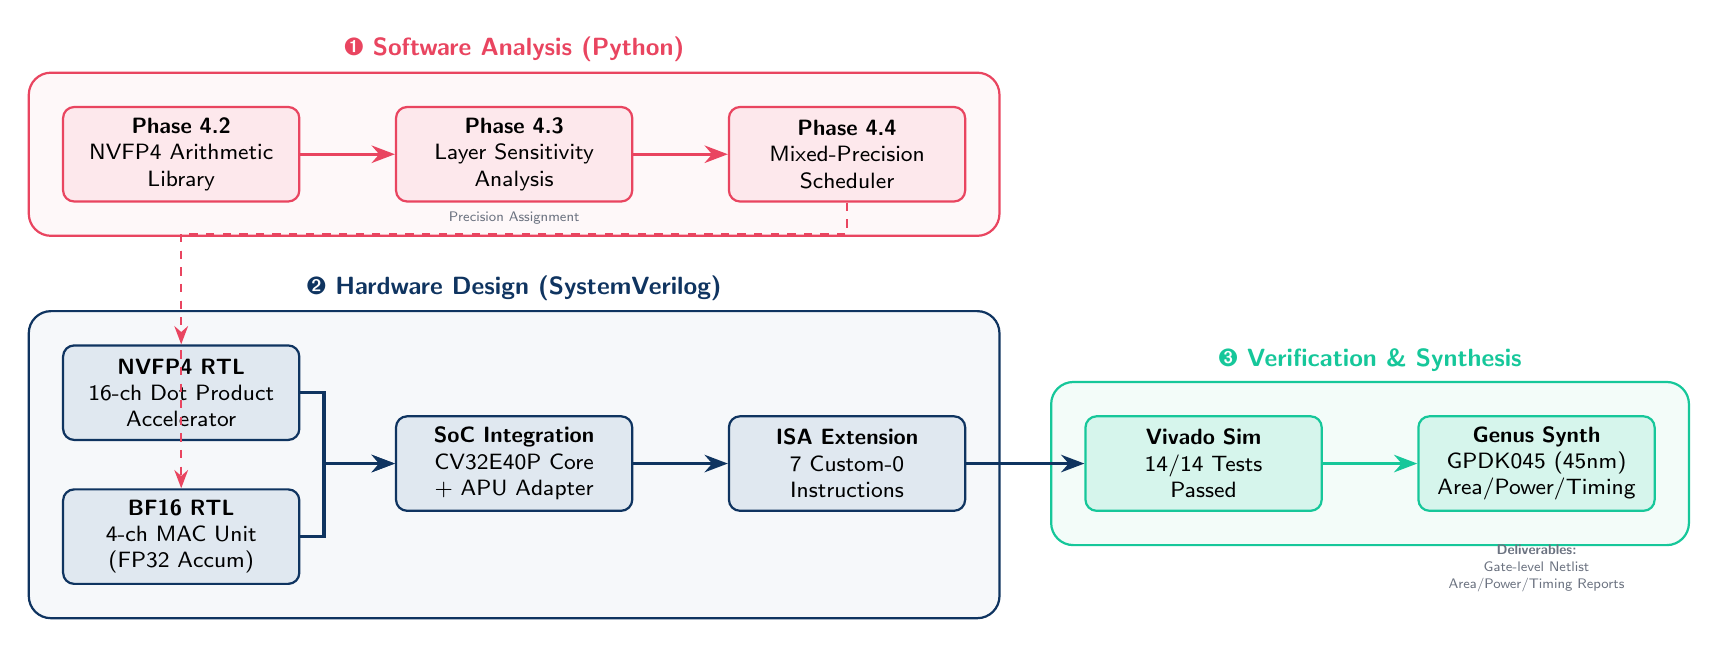
\begin{tikzpicture}[
    >=Stealth,
    node distance=0.6cm and 1.2cm,
    phase/.style={
        draw, rounded corners=4pt, minimum width=3.0cm, minimum height=1.2cm,
        font=\footnotesize\sffamily, align=center, thick, text width=2.6cm
    },
    swphase/.style={phase, fill=swRedLt, draw=swRed},
    hwphase/.style={phase, fill=hwBlueLt, draw=hwBlue},
    verphase/.style={phase, fill=verGreenLt, draw=verGreen},
    groupbox/.style={draw, rounded corners=8pt, thick, inner sep=12pt},
    dashed arrow/.style={->, thick, dashed, arrowGray},
]

% ============================================
% Software Analysis
% ============================================
\node[swphase] (arith) {\textbf{Phase 4.2}\\NVFP4 Arithmetic\\Library};
\node[swphase, right=of arith] (sens) {\textbf{Phase 4.3}\\Layer Sensitivity\\Analysis};
\node[swphase, right=of sens] (sched) {\textbf{Phase 4.4}\\Mixed-Precision\\Scheduler};

\begin{scope}[on background layer]
\node[groupbox, fill=swRedLt!30, draw=swRed,
      fit=(arith)(sens)(sched),
      label={[font=\small\sffamily\bfseries, text=swRed]above:\ding{202} Software Analysis (Python)}] (swbox) {};
\end{scope}

\draw[->, very thick, swRed] (arith) -- (sens);
\draw[->, very thick, swRed] (sens) -- (sched);

% ============================================
% Hardware Design
% ============================================
\node[hwphase, below=1.8cm of arith] (nvfp4) {\textbf{NVFP4 RTL}\\16-ch Dot Product\\Accelerator};
\node[hwphase, below=0.6cm of nvfp4] (bf16) {\textbf{BF16 RTL}\\4-ch MAC Unit\\(FP32 Accum)};
\node[hwphase, right=of nvfp4, yshift=-0.9cm] (soc) {\textbf{SoC Integration}\\CV32E40P Core\\+ APU Adapter};
\node[hwphase, right=of soc] (isa) {\textbf{ISA Extension}\\7 Custom-0\\Instructions};

\begin{scope}[on background layer]
\node[groupbox, fill=hwBlueLt!30, draw=hwBlue,
      fit=(nvfp4)(bf16)(soc)(isa),
      label={[font=\small\sffamily\bfseries, text=hwBlue]above:\ding{203} Hardware Design (SystemVerilog)}] (hwbox) {};
\end{scope}

\draw[->, very thick, hwBlue] (nvfp4.east) -- ++(0.3,0) |- (soc.west);
\draw[->, very thick, hwBlue] (bf16.east) -- ++(0.3,0) |- (soc.west);
\draw[->, very thick, hwBlue] (soc) -- (isa);

% ============================================
% Verification & Synthesis
% ============================================
\node[verphase, right=1.5cm of isa] (vivado) {\textbf{Vivado Sim}\\14/14 Tests\\Passed \checkmark};
\node[verphase, right=of vivado] (genus) {\textbf{Genus Synth}\\GPDK045 (45nm)\\Area/Power/Timing};

\begin{scope}[on background layer]
\node[groupbox, fill=verGreenLt!30, draw=verGreen,
      fit=(vivado)(genus),
      label={[font=\small\sffamily\bfseries, text=verGreen]above:\ding{204} Verification \& Synthesis}] (verbox) {};
\end{scope}

\draw[->, very thick, verGreen] (vivado) -- (genus);

% ============================================
% Cross-phase connections
% ============================================
\draw[dashed arrow, swRed] (sched.south) -- ++(0,-0.4) -| node[pos=0.25, above, font=\tiny\sffamily, text=arrowGray] {Precision Assignment} (nvfp4.north);
\draw[dashed arrow, swRed] (sched.south) -- ++(0,-0.4) -| (bf16.north);
\draw[->, very thick, hwBlue] (isa.east) -- ++(0.5,0) |- (vivado.west);

% ============================================
% Output labels
% ============================================
\node[font=\tiny\sffamily, text=arrowGray, below=0.3cm of genus, align=center] {
    \textbf{Deliverables:}\\
    Gate-level Netlist\\
    Area/Power/Timing Reports
};

\end{tikzpicture}
\end{document}
